%! Author = melek
%! Date = 29.12.2022

% Preamble
\documentclass[11pt]{article}

% Packages
\usepackage{amsmath}
\usepackage{graphicx}
\graphicspath{ {../images/} }

\title{Assignment 2: Policy Gradients}
\author{huseyinabanox@gmail.com}
\date{January 2023}

% Document
\begin{document}

    \maketitle

    \section{Small-Scale Experiments}

    \subsection{Experiment 1}

    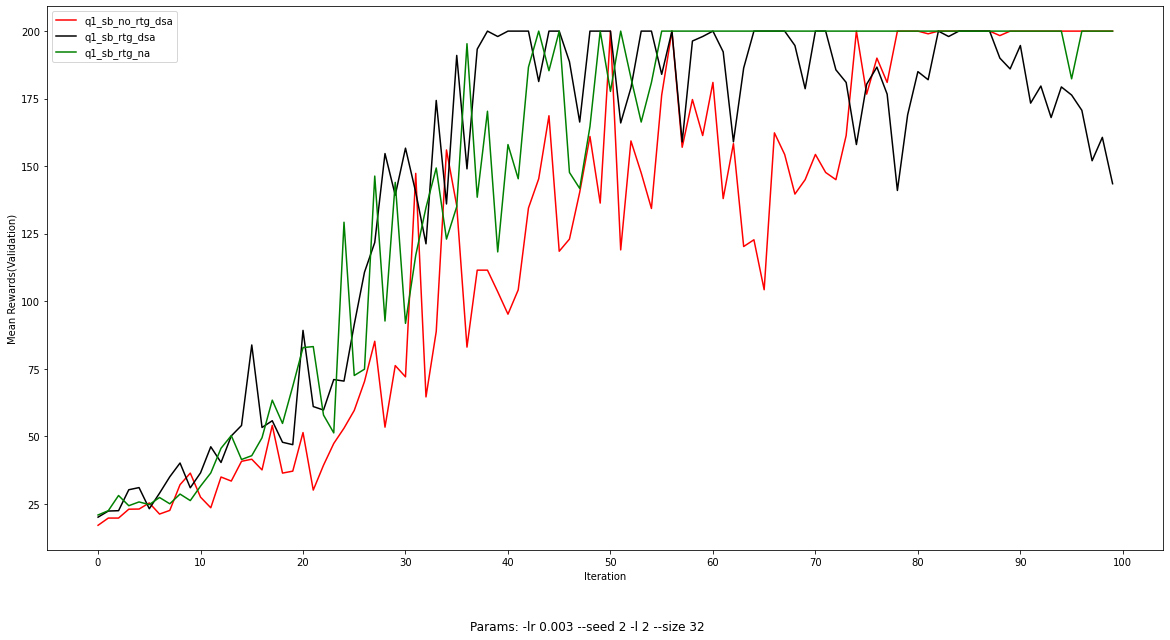
\includegraphics[scale=0.35]{q1/q1_sb_plot}

    Reward-to-go estimator performs better.
    Advantage standardization difference is not statistically significant.


    \hspace*{-0.5in}
    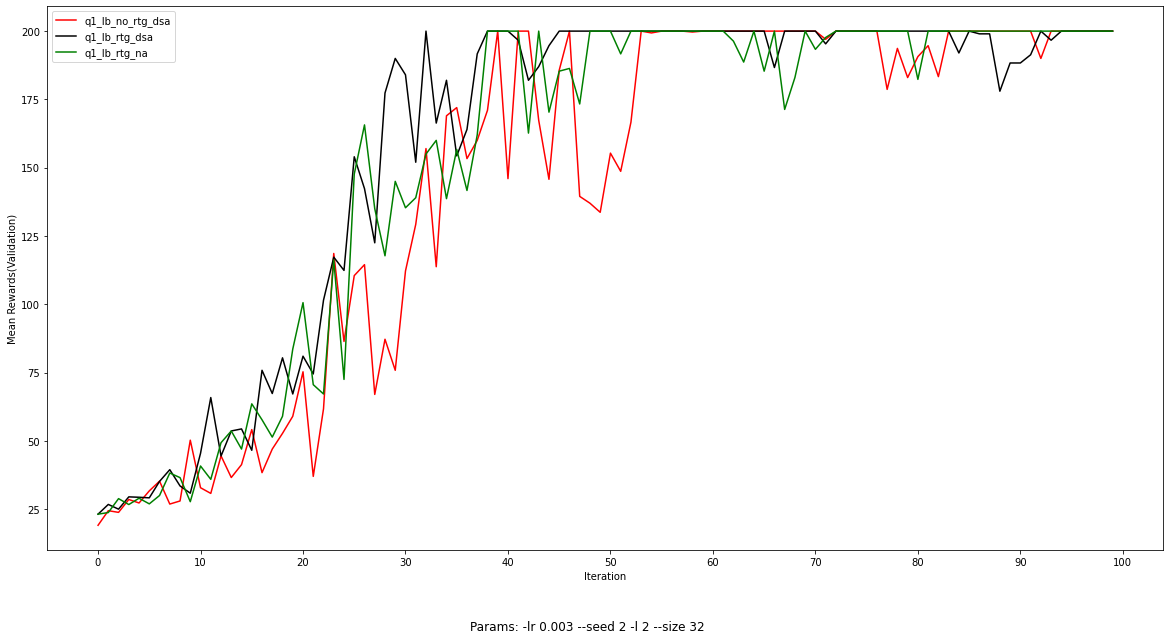
\includegraphics[scale=0.35]{q1/q1_lb_plot}

    Reward-to-go estimator performs better.
    Advantage standardization difference is not statistically significant.
    Increasing the batch size helps the trajectory-centric algorithm converge with fewer iterations.


    \subsection{Experiment 2}

    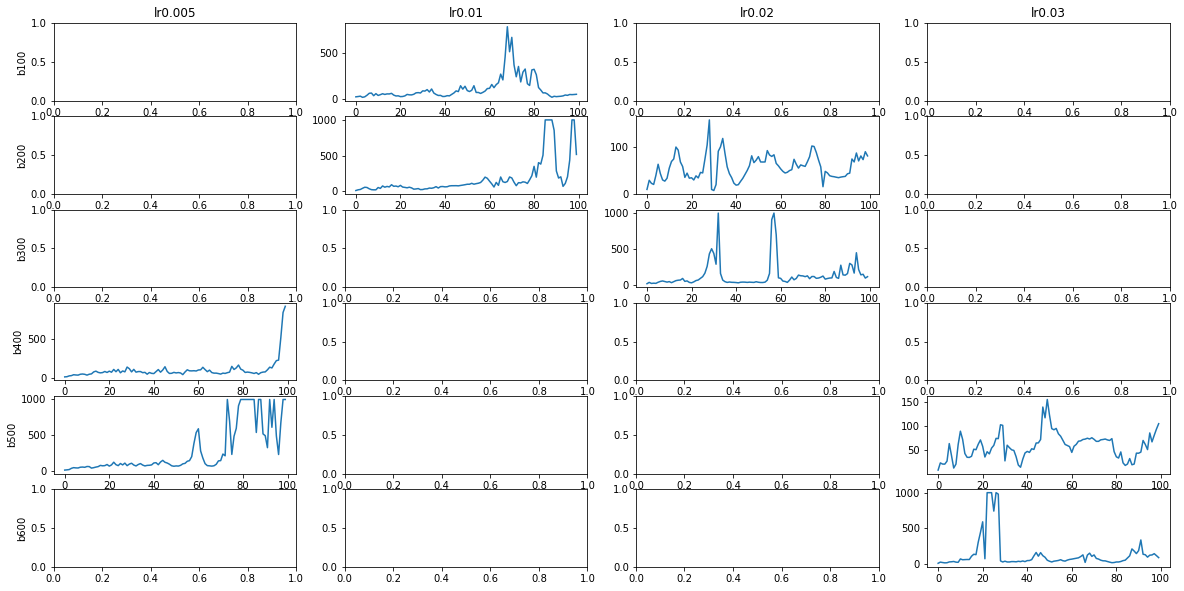
\includegraphics[scale=0.35]{q2_grid_plot}

    A grid search with default parameters shows that it is possible to reach the target reward of 1000 with learning rate 0.01 and batch size 200 or with learning rate 0.02 and batch size 300.
    The first options seems to be more stable.

    Please note that the figure tries to show the boundary in hyperparameter space.
    In each column the first chart indicates largest learning rate and smallest batch size that fails to reach 1000.
    In each column the second chart indicates largest learning rate and smallest batch size that succeeds in reaching 1000.

\end{document}